
\section*{TEE Identification and Attestation}

Remote attestation is one of the key features of enclave architectures like SGX. In remote attestation, an external verifier wants to check that an enclave was constructed as expected. To do this, the verifier sends a challenge to the attested CPU. The CPU signs the challenge together with a previously recorded measurement of the enclave's code and setup sequence using a processor-specific attestation key. The signature can also include application-specific data, such as the public key of the enclave, that later allows secure communication with the attested enclave. The attestation key is part of a group signature scheme that is managed by Intel. The signed attestation statement is then sent back to the verifier. If the attestation signature can be verified correctly, the remote verifier knows that the attested enclave was correctly constructed and runs the expected code inside a legitimate SGX processor. 

In many applications, secure computation alone is insufficient. What is rather needed is a way to check in what kind of protected environment this computation is or was performed. Remote attestation achieves exactly this property, and thus, it is a very useful feature for many enclave deployment scenarios. For example, remote attestation allows external entities to verify the correctness of enclaves before provisioning secrets to them or before accepting signed messages from them.  

\subsubsection*{Relay Attacks}

The above-explained attestation scheme has a known weakness. %As is shown in Figure~\ref{fig:SystemModel}, 
An adversary that controls the OS on the attested computing platform can easily \emph{re-direct} the attestation request to another, similar platform that computes the expected attestation response. 

The remote verifier cannot notice such \emph{relay attacks}, since the attestation mechanism is based on a group signature scheme, and all processors that are part of the same group produce indistinguishable signatures. (Even if attestation signatures were traditional digital signatures, it would be very difficult, in practice, for the verifier to know which signing key corresponds to which CPU.) 

%\begin{figure}[t]
%    \centering
%    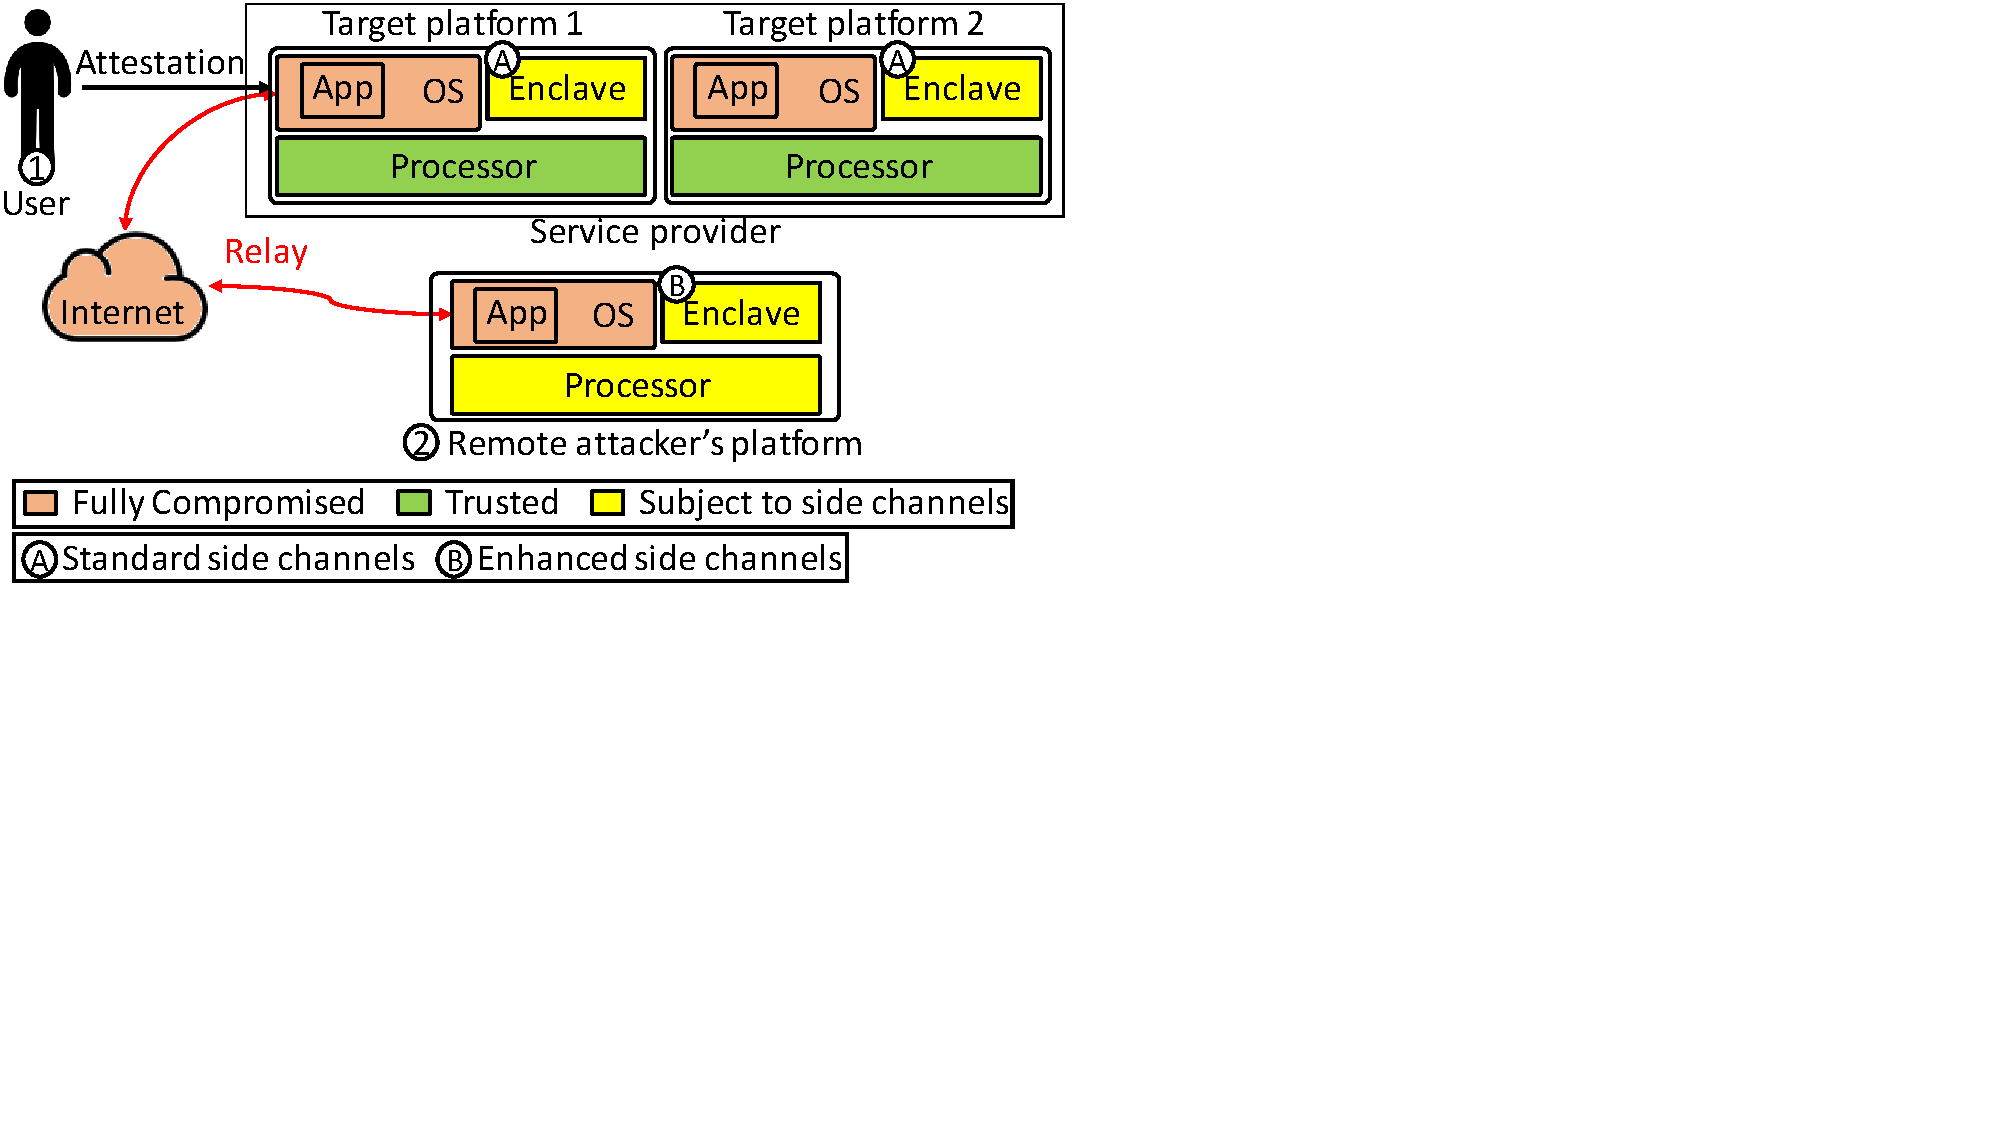
\includegraphics[trim={0cm 9cm 15.8cm 0},clip,width=0.8\linewidth]{relayAttack2.pdf}
%    \caption{Attestation relay attack. An adversary that controls the OS on the target platform re-directs the attestation to another platform.}
%    \label{fig:SystemModel}
%\end{figure}

Relay attacks have been known for a long time. Parno identified them in the context of TPM attestation over a decade ago and called them ``cuckoo attacks''~\cite{parno2008bootstrapping}. However, the full implications of relay attacks have not been well understood. Since attestation can only be redirected to another legitimate processor, it may appear that such relay attacks do not have noteworthy negative implications. Our analysis shows that such a belief is misguided.

\begin{figure}[t]
\footnotesize
    \centering
    \begin{tikzpicture}[
solved/.style={rectangle,draw,fill=purple!40, rounded corners, align=center},
not/.style={rectangle, draw,fill=orange!60, rounded corners, align=center},
neutral/.style={rectangle, draw, rounded corners, align=center, fill=black!5},
sibling distance=12em]]
    \node[neutral](root) {SGX attacks}
    child { node[not, yshift=13pt] (name) {Attacks enabled by \\ leaked attestation keys ~\cite{van2018foreshadow}} }
    child { node[neutral, yshift=13pt] (app) {Side-Channels \\ on application enclave}
      child { node[neutral, yshift=12pt] (soft) {Software/digital}
        child { node[solved, yshift=-4pt] (pe) {Privilege\\ escalation}}      
        child { node[not, right=1.5em of pe] (a) {Complement of Case (A)}}
        child { node[solved, right=1.5em of a, yshift=-10pt] {Case (A):\\
                Target platform: secure\\
                Attacker's platform: vulnerable}}}
      child { node[solved, yshift=12pt] (physical) {Physical} } };
      
    %\node[below=0cm of name] {Foreshadow~\cite{foreshadow-usenix18}};
    \node[below=0cm of physical](power) {Power analysis}; %~\cite{wang2006covert}};
    \node[below=-5pt of power](EM) {EM radiation}; %~\cite{gandolfi2001electromagnetic}};
    \node[below=-5pt of EM](ac) {Acoustic}; %~\cite{shamir2004acoustic}};
         
    \node[left=10pt of soft](page) {Page fault}; %~\cite{xu2015controlled}};
    \node[above=-3pt of page](cache) {Cache}; %~\cite{dall2018cachequote}};
    \node[below=-2pt of page](branch) {Branch prediction}; %~\cite{lee2017inferring}};
    %\node[below=-5pt of branch](synch) {Synchronization~\cite{asyncshock}};
      
    \node[solved, right=4em of root,  minimum size=3mm](l1) {};
    \node[right=0cm of l1](l1_1) {Enabled by relay};
    \node[not, below=1pt of l1, minimum size=3mm](l2) {};
    \node[right=0cm of l2](l2_1) {Independent of relay};
    
    \end{tikzpicture}
    
    \caption{Relay attack implications. Classification of attacks that are enabled by relaying and independent of relaying.}
    \label{fig:relayTree}
\end{figure}            

\paragraph{Relay attack implications}
The main implication of relay attacks is that they \emph{increase} the adversary's ability to attack the attested enclave. As is illustrated in Figure~\ref{fig:relayTree}, the first major adversarial benefit is that by redirecting the attestation to a platform that in the permanent possession of the adversary, the adversary enables \emph{physical} side-channel attacks such as acoustic, electric and electromagnetic monitoring, which have been shown to be both effective and inexpensive means to extract secrets from modern PC platforms~\cite{genkin2016physical}. Hardening enclaves against physical side channels is very difficult. 

Another benefit of relay attacks is that it can enable \emph{privilege escalation}. In cases where the adversary has only compromised the user-space application that manages the enclave, and not the OS, the application can redirect the attestation to the attacker's remote platform where he controls the OS as well. In such cases, the relay enables \emph{digital} side-channel attacks that require system privileges.

The third, and perhaps most subtle, implication of relay is that it can enable software-based side-channel attacks that would not be otherwise possible due to \emph{timing} of certain events. One such example is a scenario where the OS is compromised at the time of attestation and secret provisioning, and the enclave is hardened against known digital side-channel attacks (e.g., using tools like Raccoon~\cite{raccoon}). After secret provisioning, the OS compromise is detected and cleaned. Later, a new side-channel attack vector (that is not prevented by the used tools) is discovered. If the adversary performed redirection during attestation and the secret was provisioned to the attacker's machine, the new side-channel is exploitable. Without the relay, the attack is not possible. See Case(A) in the attack classification tree of Figure~\ref{fig:relayTree}.

We note that attacks based on leaked attestation keys (e.g., ones obtained through the Foreshadow attack~\cite{van2018foreshadow}) are independent of relaying. If the adversary has obtained a valid and non-revoked attestation key, he can emulate an SGX processor on the target platform and steal any secrets that are provisioned to it.


\subsubsection*{\proximitee System}

Parno identified relay attacks more than a decade ago and, at the same time, suggested \emph{proximity verification} as a solution~\cite{parno2008bootstrapping}. The main idea was to verify that the attested CPU is in the proximity of the verifier, which should prevent attestation redirection to another remote platform. 

Although this idea sounds simple to realize, the research efforts that followed failed to implement secure proximity verification. The main reason for the failure was that TPM, the secure element that was commonly available at the time, supported only fixed identification operations like digital signatures. TPM signatures may take up to one second, which allows the redirected attestation request to travel a long distance, and thus TPMs were simply too slow for secure proximity verification implementation. %~\cite{CatchingCuckoo}.

Because SGX enclaves are programmable, it is possible to implement proximity verification protocols that leverage simple operations like \texttt{XOR} that enable fast challenge-response rounds. Based on this observation, we designed a hardened SGX attestation scheme, called \proximitee~\cite{proximitee}. %, that is illustrated in Figure~\ref{fig:proximitee}. 
\red{One strawman solution is to use the SGX local attestation using a challenger enclave. This will prove if the application enclave and the challenger enclave are running on the same platform. But this solution won't work because deploying the challenger enclave requires attestation to that enclave where the attacker can mount the relay attack. Hence, only way to solve the problem is to introduce a trusted device that is \emph{external} to the platform to prove the proximity}
Our solution uses a simple embedded device that we call \key. The embedded device is attached to the target platform over a local communication interface such as USB. The \key device first performs standard remote attestation on the local enclave, then it establishes a secure channel like TLS connection to it, and verifies the proximity of the attested enclave using a simple distance bounding protocol that consist of repeated and fast challenge-response rounds. If such proximity verification succeeds, \key facilitates the creation of a secure channel between the remote verifier and the attested enclave. 

%\begin{figure}[t]
% \centering
%  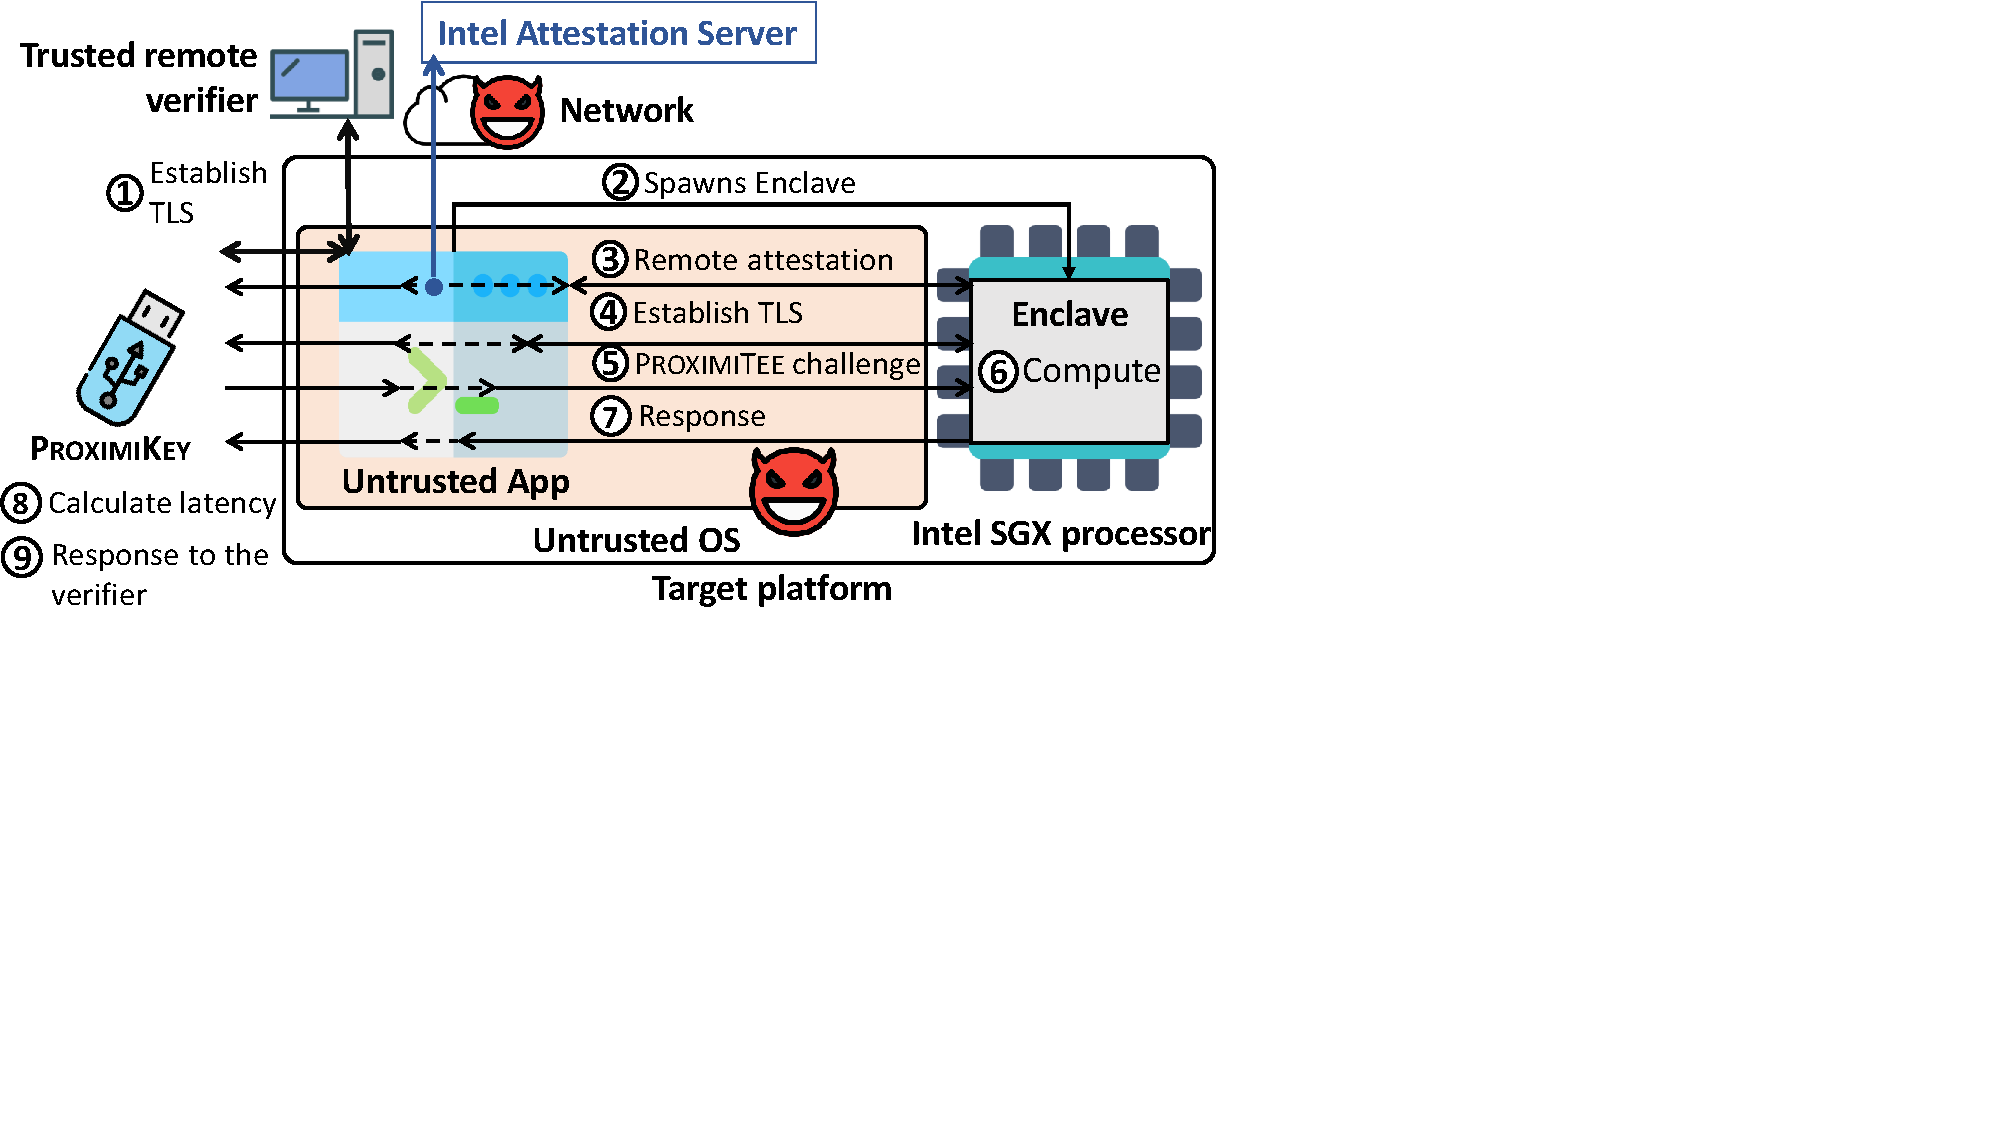
\includegraphics[trim={0 8.7cm 13.2cm 0},clip,width=\linewidth]{proximiteeMain.pdf}
% \caption{\proximitee system. The remote verifier establishes a secure channel to the \key device that first attests the enclave and then verifies its proximity.}
% \label{fig:proximitee}
%\end{figure}

%The \proximitee attestation protocol that proceeds as shown in Figure~\ref{fig:proximitee}: \one The remote verifier establishes a secure channel (e.g., a TLS connection) to \key based on a device certificate that it learned from its issuer. \two The enclave is started and \three the \key device performs the standard remote attestation to verify the code configuration of the enclave, and in the process, it learns the public key of the attested enclave. \four The \key device establishes a secure channel to the enclave using that public key. 

%\five \key performs a distance-bounding protocol that consists of several rounds. At the beginning of each round, \key generates a random challenge and sends it to the enclave over the TLS channel. \six The enclave increments the received challenge by one and \seven sends the response back to the \key that \eight verifies that the response value is as expected and checks if the latency of the response is below a threshold. Successful proximity verification requires that the latency is below a specific threshold for sufficiently many responses. \nine  If proximity verification is successful, the \key notifies the remote verifier who can now establish a secure channel to the verified enclave.

\paragraph{Proximity verification security} While the above design of the \proximitee system is mostly straightforward, the more interesting aspect is whether such a system prevents relay attacks in practice. To answer this question, we implemented our solution using a USB prototyping board and simulated a strong attack scenario where the adversary performs a relay to another SGX platform that is connected to the target platform over a one-meter long Ethernet wire. We also assumed that the adversary is able to perform all protocol computation instantaneously. 

\begin{figure}[t]
  \centering
    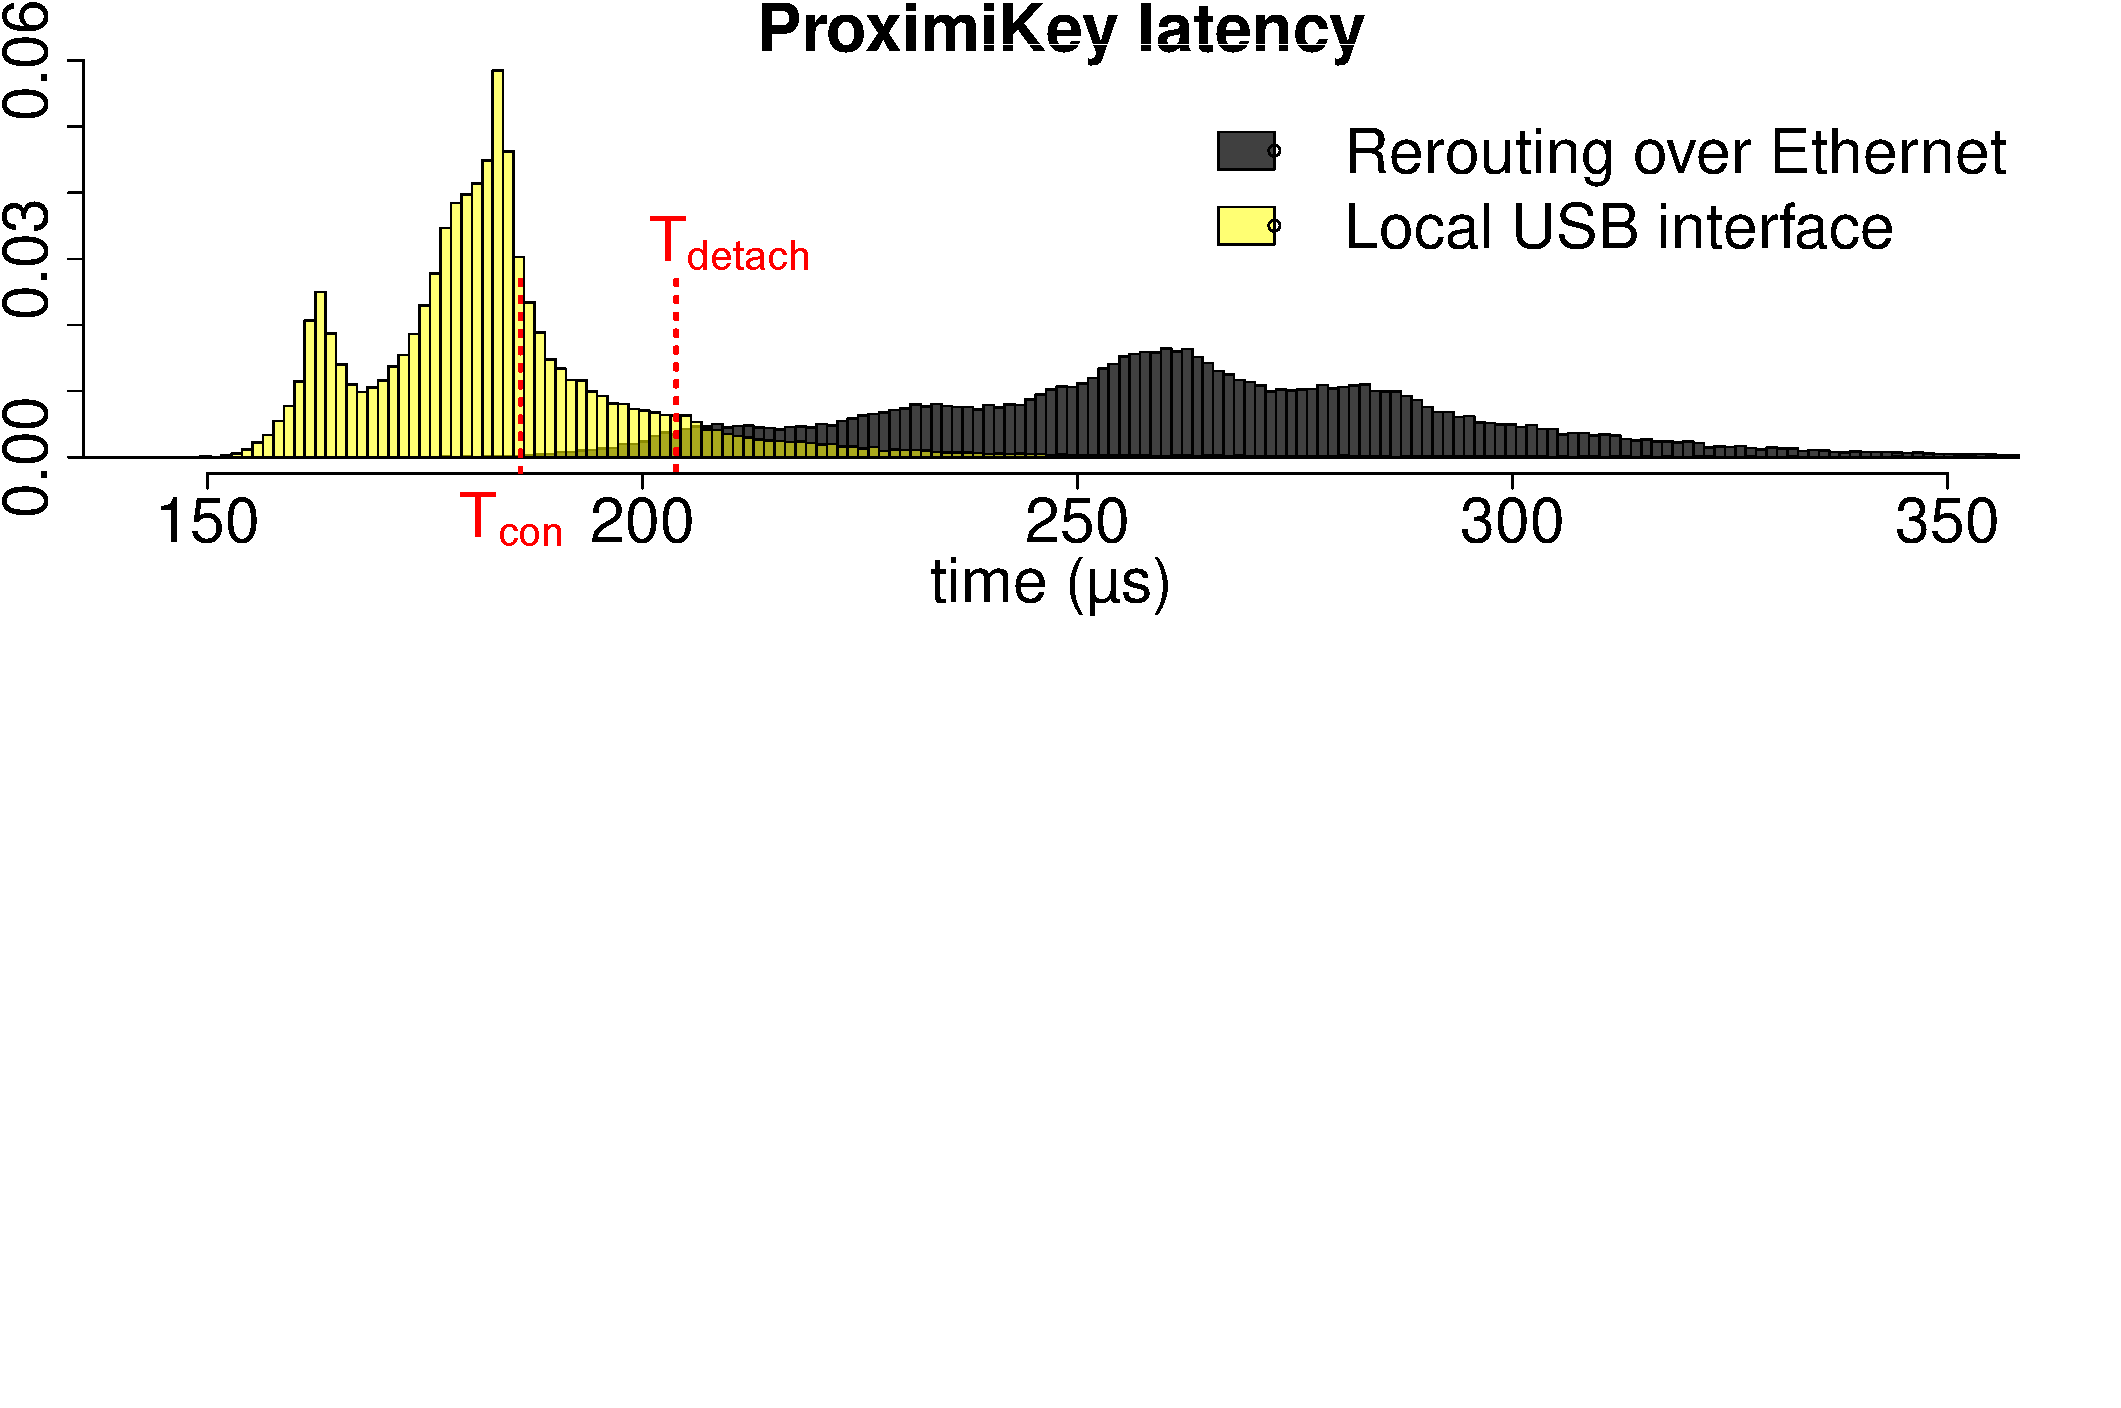
\includegraphics[trim={0 13.4cm 0 0},
    clip,width=\linewidth]{histo.pdf} 
    \caption{Latency distributions for legitimate challenge-response rounds and simulated relay attack.}
    \label{graph:histogram}
\end{figure}

Figure~\ref{graph:histogram} shows the results from our experiments, where we measured both the legitimate and relayed challenge-response latencies. The vast majority of the benign latencies range from $145$ to $250 \mu s$, while the attack round-trips take from $200$ to $750$ $\mu s$. The average delay of our adversary is only $80 \mu s$. To put this into perspective, even the highly-optimized network connections between major data centers in the same region exhibit latencies from one millisecond upwards, which is one order of magnitude more than in our simulated setup. 

As can be seen from Figure~\ref{graph:histogram}, these two latency distributions are clearly distinguishable. Our analysis confirms that it is possible to set protocol parameters (number of challenge-response rounds, latency threshold, etc.) such that even very fast relay attacks can be detected with high probability and legitimate attestations fail only with negligible probability. The full details of the \proximitee system and our analysis can be found from~\cite{proximitee}.

%We simulate a powerful relay-attack adversary that is connected to the target platform with a fast network connection. To consider the best case for the adversary, we make several assumptions in his favor. For example, we assume that he can instantly perform all computations needed to participate in the proximity verification protocol. However, he cannot break cryptographic hardness assumptions. We define the adversary's success as the event in which proximity verification succeeds with an enclave that resides on the attacker's platform and denotes the probability of such event $P_{adv}$. We define legitimate success as the event in which proximity verification succeeds with an enclave that resides in the target platform and denotes its probability $P_{legit}$. We saw that it is possible to find parameters ($n=50$, $k=0.3$ and \proximitee$=186 \mu s$) that make proximity verification very secure ($P_{adv}=3.55\times 10^{-34}$) and reliable ($P_{legit}=0.999999977$).




